\documentclass[tikz,border=5pt]{standalone}
\usepackage[T1]{fontenc}
\usepackage{lmodern,amsmath,amssymb}
\usetikzlibrary{arrows.meta,calc,positioning,fit,backgrounds,shapes.geometric,matrix,decorations.pathreplacing,patterns}
\definecolor{ink}{gray}{0.08}
\definecolor{wash}{gray}{0.965}
\definecolor{soft}{gray}{0.45}
\tikzset{box/.style={draw=ink,line width=.65pt,fill=white,align=center,inner sep=4pt,outer sep=0pt,font=\small},flow/.style={draw=ink,line width=.65pt,-{Latex[length=1.8mm,width=1.3mm]},rounded corners=2pt},annotation/.style={font=\scriptsize,text=soft,align=center},groupbox/.style={draw=soft,dashed,line width=.45pt,fill=wash}}
\begin{document}
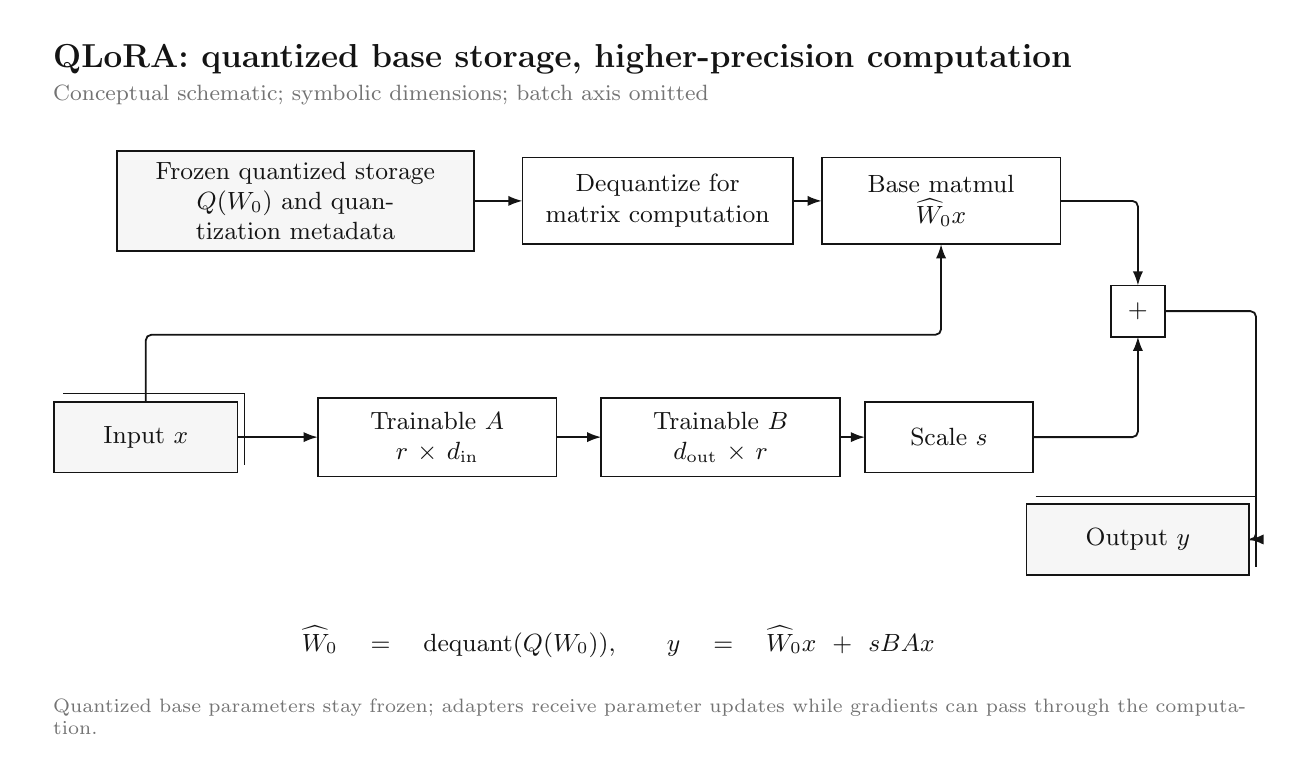
\begin{tikzpicture}[x=1cm,y=-1cm,font=\rmfamily,text=ink]

\path[use as bounding box] (0,0) rectangle (16,9);
\node[anchor=west,font=\large\bfseries] at (.2,.4) {QLoRA: quantized base storage, higher-precision computation};
\node[anchor=west,font=\footnotesize,text=soft] at (.2,.85) {Conceptual schematic; symbolic dimensions; batch axis omitted};
\begin{pgfonlayer}{background}
\end{pgfonlayer}
\node[box,fill=wash,minimum width=4.5cm,minimum height=1.1cm,text width=4.25cm] (qw) at (3.4,2.2) {Frozen quantized storage\\$Q(W_0)$ and quantization metadata};
\node[box,minimum width=3.4cm,minimum height=1.1cm,text width=3.15cm] (dq) at (8,2.2) {Dequantize for\\matrix computation};
\node[box,minimum width=3.0cm,minimum height=1.1cm,text width=2.75cm] (base) at (11.6,2.2) {Base matmul\\$\widehat W_0x$};
\node[box,fill=wash,minimum width=2.3cm,minimum height=0.9cm,text width=2.05cm] (x) at (1.5,5.2) {Input $x$};
\draw[ink,line width=.4pt] (0.45000000000000007,4.65) -- (2.75,4.65) -- (2.75,5.550000000000001);
\node[box,minimum width=3.0cm,minimum height=1.0cm,text width=2.75cm] (a) at (5.2,5.2) {Trainable $A$\\$r\times d_{\rm in}$};
\node[box,minimum width=3.0cm,minimum height=1.0cm,text width=2.75cm] (b) at (8.8,5.2) {Trainable $B$\\$d_{\rm out}\times r$};
\node[box,minimum width=2.1cm,minimum height=0.9cm,text width=1.85cm] (scale) at (11.7,5.2) {Scale $s$};
\node[box,minimum width=0.65cm,minimum height=0.65cm,text width=0.4cm] (add) at (14.1,3.6) {$+$};
\node[box,fill=wash,minimum width=2.8cm,minimum height=0.9cm,text width=2.55cm] (out) at (14.1,6.5) {Output $y$};
\draw[ink,line width=.4pt] (12.799999999999999,5.95) -- (15.6,5.95) -- (15.6,6.8500000000000005);
\node[align=center,inner sep=0pt,outer sep=0pt,font=\small,minimum width=13cm,minimum height=0.7cm,text width=12.75cm] (note9) at (7.5,7.8) {$\widehat W_0=\operatorname{dequant}(Q(W_0))$,\qquad $y=\widehat W_0x+sBAx$};
\begin{pgfonlayer}{background}
\draw[flow] (qw.east) -- (dq.west);
\draw[flow] (dq.east) -- (base.west);
\draw[flow] (x.north) -- (1.5,3.9) -- (11.6,3.9) -- (base.south);
\draw[flow] (x.east) -- (a.west);
\draw[flow] (a.east) -- (b.west);
\draw[flow] (b.east) -- (scale.west);
\draw[flow] (base.east) -- (14.1,2.2) -- (add.north);
\draw[flow] (scale.east) -- (14.1,5.2) -- (add.south);
\draw[flow] (add.east) -- (15.6,3.6) -- (15.6,6.5) -- (out.east);
\end{pgfonlayer}
\node[anchor=west,align=left,font=\scriptsize,text=soft,text width=15.6cm] at (.2,8.75) {Quantized base parameters stay frozen; adapters receive parameter updates while gradients can pass through the computation.};
\end{tikzpicture}
\end{document}
